% !TEX root = ./main.tex
\section*{Supplementary Material}

\section{Additional details for Section \ref{sec:problem-statement}}
\label{sec:problem-statement-app}
\noindent
\textbf{Influence Maximization.} In the Influence Maximization (\infmax) problem \cite{kempe:sigkdd03}, we are given a directed graph $G=(V,E)$ and edge weights $p(u, v) \in [0, 1]$ indicating the probability that node $u$ influences node $v$. The goal is to find a set $S \subset V$ of $k$ \emph{seed nodes} to infect, such that the expected number of influenced nodes or \emph{spread}, $\sigma(S)$, is maximized. A commonly-used diffusion process in the IM problem is the Independent Cascade model \cite{kempe:sigkdd03}, in which each recently-influenced node $u$ has one chance to influence each neighbor $v$, succeeding with probability $p(u,v)$.
Note that an instance of \infmax{} consists only of a contact graph $G$, whereas an instance of \maxcrit{} consists of the contact graph $G$, a partition of the nodes of $G$ into regions, $\R$, and an
auxiliary graph $H_{\R}$ that captures connectivity among $\R$.

\begin{theorem}
%\label{theorem:nphard}
\maxcrit{} is NP-hard. 
\end{theorem}

\begin{proof}
\infmax{} is polynomial-time reducible to \maxcrit{}, which implies the NP-hardness, since \infmax{} is NP-hard. We construct a suitable auxiliary graph $H_{\R}$ and a vaccination vector $\mathbf{x}$, showing that the spread from the Independent Cascade model in the instance of \infmax{} is stochastically equivalent to the SEIR process in the instance of \maxcrit{}.

Suppose we are given an arbitrary instance of IM; that is, a directed graph $G_\infmax=(V_\infmax,E_\infmax)$, edge probabilities $p(u,v)$ for every edge $e=(u,v) \in E$, and parameter $k$. We will create an instance of \maxcrit{} with social contact network $G_\maxcrit = (V_\maxcrit, E_\maxcrit)$, region graph $\HR$ transmission probabilities $p'(\cdot)$, intervention $\mathbf{x}$, and parameter $k'=k+1$.

\noindent
\textbf{To construct $G_\maxcrit{}$}, we first add all the nodes and edges from $G_\infmax$. We call these nodes \emph{original}. Then, for every node $v \in V_\infmax{}$, we add a \emph{switch} node $v'$ and directed edge $(v', v)$. Additionally, we add a \emph{source} node $\src$ and undirected (or bidirectional) edges from $\src$ to each switch node $v'$.
Then, $G_\maxcrit{}$ is a graph with node set $V_\maxcrit{} = V_\infmax{} \cup \{v'| v \in V_\infmax{}\} \cup \{\src\}$ and edge set $E_\maxcrit{} = E_\infmax{} \cup \{(\src,v'), (v', \src), (v', v)|\ v \in V_\infmax{}\}$. Obviously, this construction can be performed in polynomial time in $G_\infmax{}$.

\noindent
\textbf{To construct $\HR$}, we define a set of regions $\R = \{r_v | v \in V_\infmax{}\} \cup \{r_\src\}$. That is, we have one region for each original node, plus one region for the source node. The nodes $v$ and $v'$ in $G_\maxcrit{}$ are associated with a corresponding region in $\HR$: $\loc(v)=\loc(v') = r_v$, for each $v,v'\in V_\maxcrit{}$; similarly, $\loc(\src) = r_\src$. Then, we let the graph $\HR$ be a star with center $r_\src$.

\noindent
\textbf{For the transmission probabilities}, we let $p'(u, v) = p(u,v)$, for all $e=(u,v) \in E_\infmax{}$.
Every edge from $v'$ to $v$ infects $v$ with probability 1; that is, $p'(v',v) = 1$, for all original nodes $v$. Similarly, $p'(\src, v') = p'(v', \src) = 1$, for all switch nodes $v'$.

\noindent
\textbf{The intervention vector} $\mathbf{x}$ is defined as follows. 
First, all the original nodes are left unvaccinated: $x_v = 0$, for all $v$. Second, all the switch nodes are vaccinated with probability 1: $x_{v'} = 1$, for all $v'$. Lastly, the source node $\src$ is unvaccinated, i.e., $x_{\src}=0$. 

\noindent
\textbf{Correspondence between Independent Cascade and SEIR.} Now, let $S_\infmax{}$ be a set of $k$ seed nodes in the instance of IM, and let $S_\maxcrit{}= \{v' | v \in S_\infmax{}\}$ be a set containing the corresponding switch nodes in the instance of \maxcrit{} constructed above. Set these switch nodes to be unvaccinated, and consider an SEIR process on the graph $G_\maxcrit{}$ in which the infectious period is 1 time step and node $\src$ is the only node infected initially. At time $t=0$, the process starts at node $\src$; then, at $t=1$, all the nodes in $S_\maxcrit{}$ are infected deterministically, and at $t=2$, all the nodes in $S_\infmax{}$---and only the nodes in $S_\infmax{}$---are infected. From here on, the SEIR process in $G_\maxcrit{}$ is stochastically equivalent to the Independent Cascade model in $G_\infmax{}$. 

\noindent
\textbf{Equivalence between instances.} To complete the proof, we claim that an instance of $\infmax{}(G_\infmax{}, k)$ is equivalent to the instance $\maxcrit{}(G_\maxcrit{}, \HR, k + 1)$.
In particular, there exists a solution $S_\infmax{}$ with spread $\sigma(S_\infmax{})$ to the former problem if and only if there exists a solution $S_\maxcrit{}$ to the latter with criticality $\crit(S_\maxcrit{}) = \sigma(S_\infmax{}) + k + 1$. 

$\Rightarrow$ Starting with $S_\infmax{}$, let $S_\maxcrit{}= \{r_v | v \in S_\infmax{}\} \cup \{r_\src\}$ be the set of corresponding regions in $\HR$, plus the region of the source node. By construction, these regions are connected in $\HR$, and $S_\maxcrit{}$ has size $|S_\infmax{}| + 1 = k + 1$, so it is a valid solution to $\maxcrit$. Furthermore, by the equivalence between Independent Cascade and SEIR, we have that $\crit(S_\maxcrit{}) = \sigma(S_\infmax{}) + k + 1$, where the $(k + 1)$ additional infections correspond to the source and switch nodes.

$\Leftarrow$ Conversely, let $S_\maxcrit{}$ be a solution to $\maxcrit{}$, which is a set of $(k+1)$ connected regions in $\HR$. Because $\HR$ is a star with $r_\src$ as its center, the node $r_\src$ has to be in $S_\maxcrit{}$; otherwise, the solution wouldn't be connected. Now, let $S_\infmax{}= \{v | r_v \in S_\maxcrit{} \setminus \{r_\src\}\}$ be the set of corresponding nodes in $G_\infmax{}$. Because $r_\src$ is in $S_\maxcrit$ and, by construction of the social contact network $G_\maxcrit{}$, the source node and $k$ switch nodes are guaranteed to be infected. After that, the SEIR process in $G_\maxcrit{}$ is equivalent to the Independent Cascade model in $G_\infmax{}$, giving us the claimed $\crit(S_\maxcrit{}) = \sigma(S_\infmax{}) + k + 1$.

%Thus, any instance of Influence Maximization under the Independent Cascade model can be viewed as an instance of \kcsp{} for the SIR process; %This completes the proof.
\end{proof}

\subsection{Impact of connectivity requirement}
The connectivity constraint has a strong effect on the solution of \maxcrit{}.
A solution computed for \infmax{} using the greedy algorithm of \cite{kempe:sigkdd03} can be arbitrarily suboptimal for the problem we propose. Informally, this follows because in \infmax{}, it is better to choose
the set of seeds to be located far apart, so that their combined influence is maximized.

\begin{observation}
%\label{obs:infmax}
There exists a family of instances $(G, H_{\R}, k)$ for which the optimum solution
$S^*$ to \maxcrit{} satisfies
$\maxcrit(S^*) =O(\frac{1}{k}\infmax(\hat{S}))$, where $\hat{S}$ is the optimum
solution to the \infmax{} version for this instance, without any connectivity requirements.
\end{observation}

For example, consider a cycle graph, as in Figure \ref{fig:observation-app}. Every node has one outgoing neighbor (clockwise direction), and every node infects its neighbor with probability 1, unless the neighbor is a blue node, in which case the probability is 0, as denoted in the figure. There are $k=4$ spreader nodes (in blue) separated by paths of length $k+1$. Consider an instance of $\infmax{}$ with size constraint $k$, and the analogous instance of $\maxcrit{}$, where, for simplicity, we assume that $G = \HR$. The optimal solution to \infmax{} consists of the $k$ hub nodes, with objective value equals to the number of nodes in the graph, $k(k+1)$, since each hub is able to propagate the infection through all the white nodes until the next clockwise hub. In contrast, the solution to \maxcrit{} must be a connected set of nodes, so the best solution would consist of a hub and the next $k$ clockwise white nodes, for an objective value of $k + 1$.

\begin{figure}
    \centering
    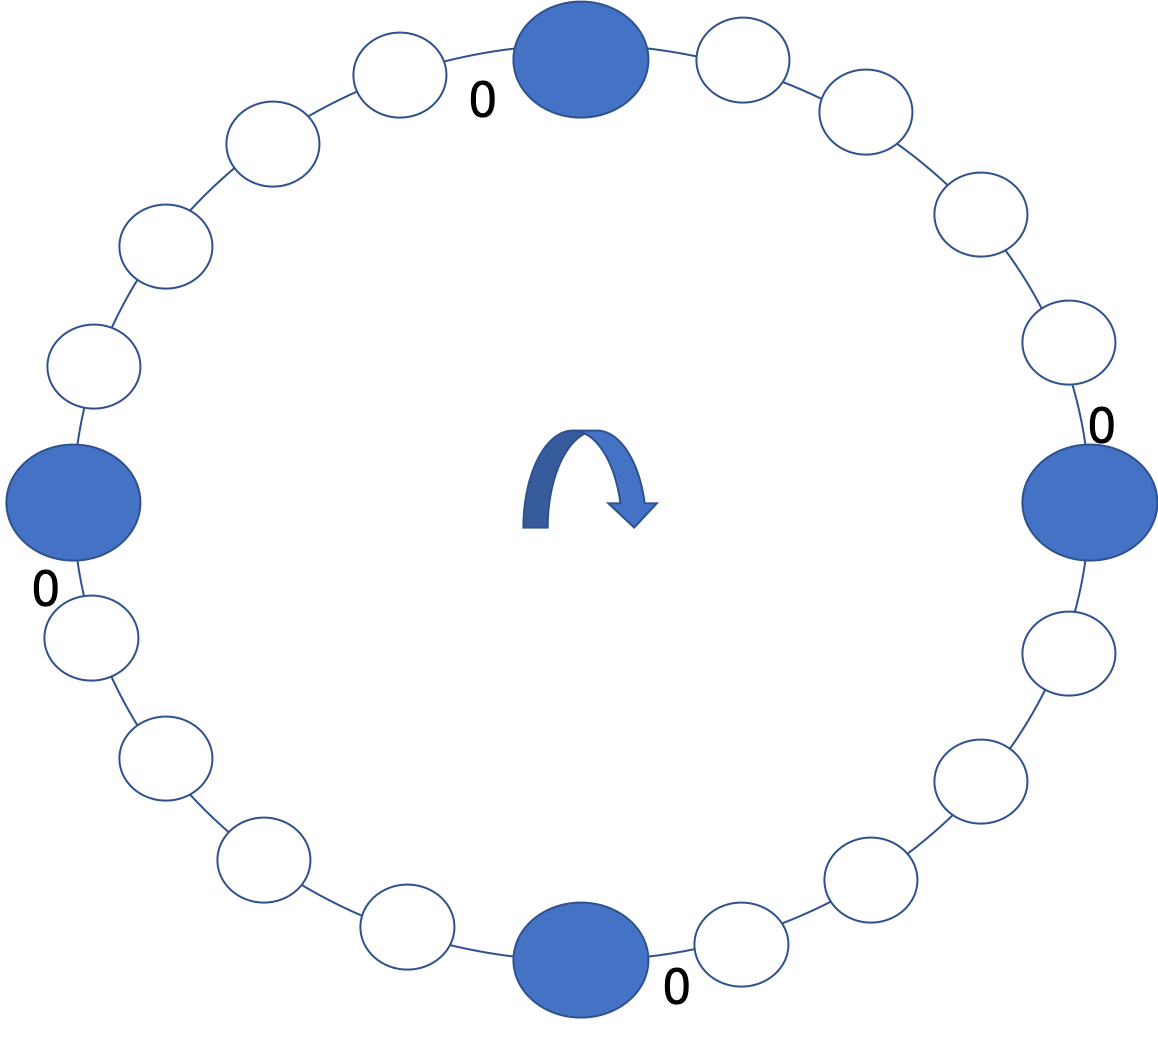
\includegraphics[width=.7\columnwidth]{img/observation.png}
    \caption{Effect of connectivity constraint in cycle graph with $k=4$ spreader nodes (blue) separated by paths of length $k + 1$. The optimal solution to $\infmax{}$ has $k$ times the objective value of the optimal solution for \maxcrit{}. See text for details.}
    \label{fig:observation-app}
\end{figure}

\section{Additional details for Section \ref{sec:proposed-critical}}
\begin{lemma}
Given a graph $G(V, E)$, $\crit(S)$ is a submodular function of $S \subset V$.
\end{lemma}

\begin{proof}
We follow the approach of Kempe et al.\ \cite{kempe:sigkdd03}, who analyze one random realization of the diffusion process at a time. For simplicity, we prove the submodularity of $\crit$ for the Independent Cascade model, but the result extends to the more general SEIR process. For each edge $e=(u,v)$, we flip a coin with bias equal to the transmission probability $p(u,v)$. Let $X(e)$ be a Bernoulli variable that is 1 with probability $p(u,v)$; then, we define the \emph{live} graph $L(V, E')$ as the subgraph of $G$ induced by the edges for which $X(e) = 1$: $L' = (V, E'=\{e \in E | X(e) = 1\})$. In the live graph, a node $v$ is infected by the end of the diffusion process if and only if $v$ is in the same component as one of the seeds in $S$. Without loss of generality, assume there is only one initial infection and let $r$ be the initially infected node. Then, the criticality of $S$ can be computed as
$$
\crit_L(S) = \left|\left(\bigcup_{s \in S} \text{comp}_L(s)\right) \cup \text{comp}_L(r)\right| - \left|\text{comp}_L(r)\right|.
$$
In words, the number of extra infections in $L$ due to node set $S$ is the size of the union of the components of nodes in $S$ minus the infections that we get if only $r$ is infected---i.e., the size of $\text{comp}_L(r)$.

Now, consider two sets $S,T$, such that $T\subseteq S$, and a node $v \not \in S$. The quantity $\crit_L(T \cup \{v\}) - \crit_L(T)$ is the number of extra infections from adding node $v$; that is, the number of elements in $\text{comp}_L(v)$ that are not already in $(\bigcup_{s \in T} \text{comp}_L(s)) \cup \text{comp}_L(r)$. This number is at least as large as the number of extra infections that we get by adding $v$ to the bigger set $S$, which gives us $\crit_L(T \cup \{v\}) - \crit_L(T) \geq \crit_L(S \cup \{v\}) - \crit_L(S)$. This is precisely the definition of submodularity, so the criticality function for a fixed live graph is submodular. Over random realizations of $L$, we obtain
$$
\crit(S) = \sum_{L}\text{Pr}(L) \crit_L(S).
$$
where $\text{Pr}(L)$ denotes the probability of obtaining the live graph $L$ with the edge probabilities $p(u,v)$. This is a convex combination of submodular functions, which is known to be submodular too, completing the proof.
\end{proof}

\subsection{Details on \greedy{} procedure and improving running time}
The $\greedy{}$ procedure in Algorithm \ref{alg:algosubmod} involves computing the criticality of every region in $\HR$ a number of times, which results in quadratic running time in the graph size. 
Instead, we use the efficient sampling approach of \cite{borgs:soda14} to significantly improve the running time. 
We call this faster procedure \textsc{FastGreedy} and show pseudocode in Algorithm \ref{alg:greedyborgs}. The inputs to \textsc{FastGreedy} are (1) the social contact network $G$, where the disease spreads, (2) a subset of regions $R\subset \R$, for which we want to find an approximate solution, (3) the vaccination vector when $R$ is undervaccinated, $\mathbf{x}^R$, and (4) the size constraint $k$. The algorithm returns a set $X \subset R$ of size $k$, just like the \greedy{} procedure. The main ideas are the following:
\begin{enumerate}
    \item We sample live graphs (defined in Section 8) until we observe at least $L=ck|E|\log{|V|}$ edges and store the components that are reachable from the source of the infection (lines 4--9)
    \item Then, we rank each node by the number of components it reaches (line 11)
    \item We form $X$ greedily by adding the $k$ nodes of highest rank, updating the ranking as we add nodes (lines 12--14) 
\end{enumerate}
As shown in \cite{borgs:soda14}, \textsc{FastGreedy} can be implemented to run in time $O(ck|E|\log{|V|})$.

\begin{algorithm}{}
\small
\caption{\small $\textsc{FastGreedy}(G=(V,E), R \subset \R, \mathbf{x}^R, k)$}
\label{alg:greedyborgs}
\begin{algorithmic}[1]
\STATE Let $\mathcal{S}=\emptyset$
\STATE Let $L=ck|E|\log{|V|}$, for a constant $c$
\STATE $\ell=0$
\WHILE{$\ell <L$}
  \STATE Pick random subgraph $G'$ of $G$ with (1) edges sampled based on
disease transmission probability, (2) nodes sampled with probability $1 - \mathbf{x}^R$
  \STATE $\ell = \ell + |E(G')|$
  \STATE Let $C_i$ be the set of components reachable from the set $\src_R$
of sources in $G'$
  \STATE $\mathcal{S} = \mathcal{S}\cup\{C_i\}$
\ENDWHILE
\STATE Initialize $X=\emptyset$
\STATE
For each $r\in R$, define $deg(r, \mathcal{S})$ to be the number
of sets $C_i\in\mathcal{S}$ that contain some node in $V(r)$
\FOR{$i=1$ to $k$}
  \STATE Append $r=\text{argmax}_{r'} deg(r',\mathcal{S})$ to $X$
\STATE
Remove all sets $C_i$ hit by $V(r)$ from $\mathcal{S}$ and update all $deg(\cdot)$
\ENDFOR
\STATE \textbf{return} $X$
\end{algorithmic}
\end{algorithm}


\begin{theorem}
\label{theorem:maxcrit-app}
If $\HR$ has doubling dimension $d$, algorithm  \algomaxcrit{} gives an $\Omega\Big(\frac{1}{k^{(d-1)/(2d-1)}}\Big)$ approximation to the \maxcrit{} problem, and it has worst case running time $O(ck^{\frac{d}{2d - 1}}|\R||E|\log{|V|} + |E_{\R}|(2e)^k)$.
\end{theorem}

\begin{proof}
The approximation guarantee follows from Theorem \ref{theorem:submod}. The running time is simply the sum of the running times of \algomaxst{} above and  \algosubmod{} implemented with \textsc{FastGreedy}. In \algosubmod{}, we invoke \textsc{FastGreedy} for each region in $\R$ using a size constraint of $\ell = k^{\frac{d}{2d - 1}}$, which gives us the claimed running time of $O(ck^{\frac{d}{2d - 1}}|\R||E|\log{|V|})$.
\end{proof}